\documentclass[tikz,border=4pt]{standalone}
\usepackage{tikz}
\usepackage{amsmath}
\usetikzlibrary{arrows.meta,calc,positioning,shapes.geometric,backgrounds,fit}

\begin{document}
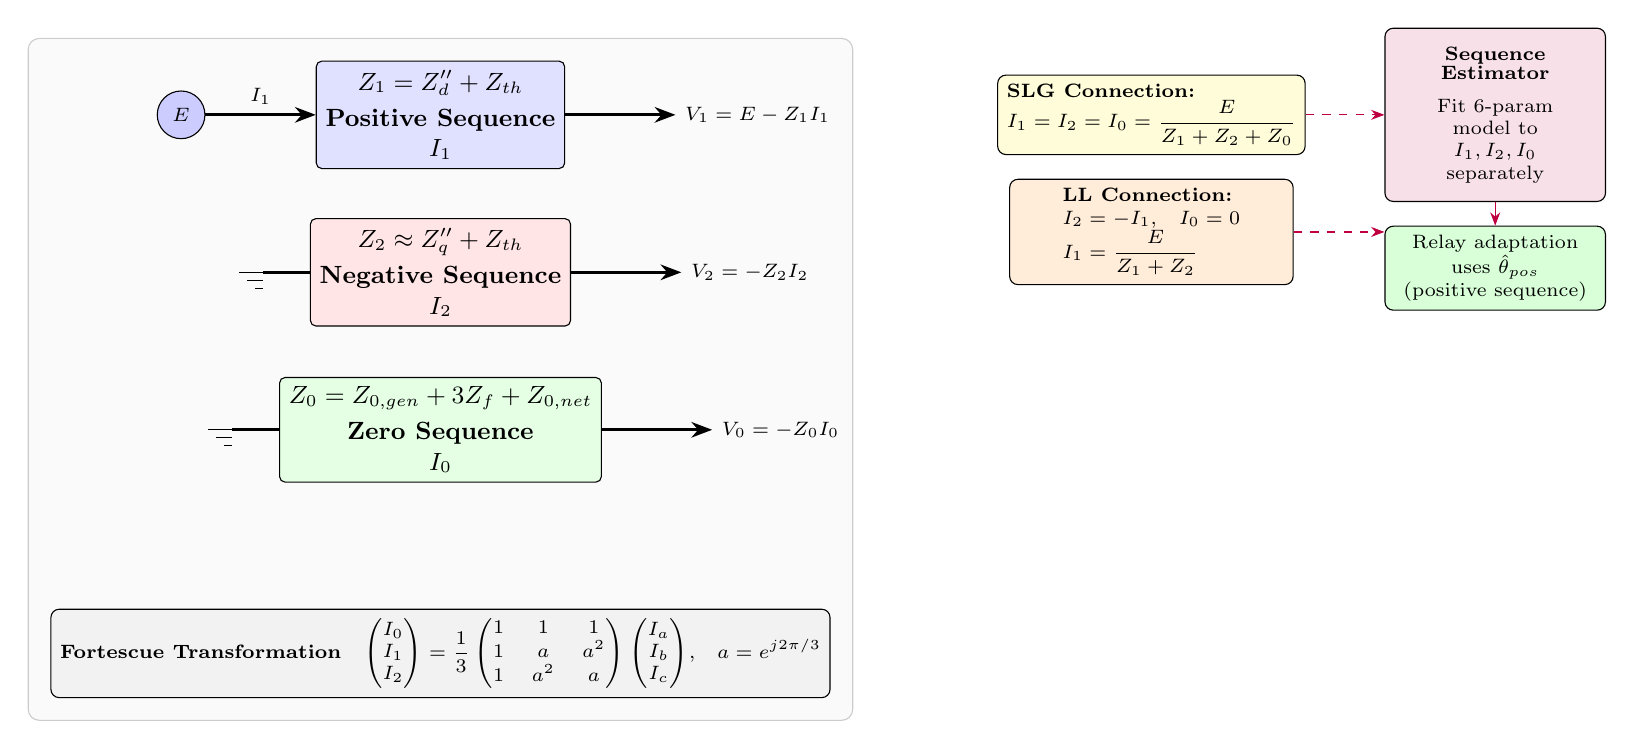
\begin{tikzpicture}[
  font=\small,
  >=Stealth,
  net/.style={draw,rectangle,minimum width=2.8cm,minimum height=1.0cm,
              align=center,rounded corners=2pt},
  wire/.style={draw,line width=1.0pt},
  label/.style={font=\scriptsize},
]

%% =====================================================
%%  THREE SEQUENCE NETWORKS stacked vertically
%%  Positive (top), Negative (middle), Zero (bottom)
%% =====================================================

% --- Positive sequence network ---
\node[net,fill=blue!12] (pos) at (0,3.5)
     {$Z_1 = Z_{d}'' + Z_{th}$\\[2pt]\textbf{Positive Sequence}\\$I_1$};

\node[draw,circle,minimum size=0.5cm,fill=blue!20,left=1.4cm of pos,
      font=\scriptsize] (vsrc1) {$E$};
\draw[wire,->] (vsrc1.east) -- node[above,label]{$I_1$} (pos.west);
\node[right=1.4cm of pos,label,align=left] (r1) {$V_1 = E - Z_1 I_1$};
\draw[wire,->] (pos.east) -- (r1.west);

% fault node at right of pos
\coordinate (fn1) at ($(r1.east)+(0.5,0)$);

% --- Negative sequence network ---
\node[net,fill=red!10] (neg) at (0,1.5)
     {$Z_2 \approx Z_{q}'' + Z_{th}$\\[2pt]\textbf{Negative Sequence}\\$I_2$};

\node[right=1.4cm of neg,label,align=left] (r2) {$V_2 = -Z_2 I_2$};
\draw[wire,->] (neg.east) -- (r2.west);

% Ground on left of neg
\coordinate (gnd2) at ($(neg.west)+(-0.6,0)$);
\draw[wire] (neg.west) -- (gnd2);
\draw (gnd2) -- ++(-0.3,0);
\draw ($(gnd2)+(0,-0.10)$) -- ++(-0.20,0);
\draw ($(gnd2)+(0,-0.20)$) -- ++(-0.10,0);

% --- Zero sequence network ---
\node[net,fill=green!10] (zero) at (0,-0.5)
     {$Z_0 = Z_{0,gen} + 3Z_f + Z_{0,net}$\\[2pt]\textbf{Zero Sequence}\\$I_0$};

\node[right=1.4cm of zero,label,align=left] (r0) {$V_0 = -Z_0 I_0$};
\draw[wire,->] (zero.east) -- (r0.west);

% Ground on left of zero
\coordinate (gnd0) at ($(zero.west)+(-0.6,0)$);
\draw[wire] (zero.west) -- (gnd0);
\draw (gnd0) -- ++(-0.3,0);
\draw ($(gnd0)+(0,-0.10)$) -- ++(-0.20,0);
\draw ($(gnd0)+(0,-0.20)$) -- ++(-0.10,0);

%% =====================================================
%%  Connection for SLG fault: I1=I2=I0
%% =====================================================
\node[draw,fill=yellow!15,rounded corners=3pt,
      right=2.0cm of r1,align=left,font=\scriptsize,minimum width=3.6cm] (slg)
      {\textbf{SLG Connection:}\\$I_1=I_2=I_0=\dfrac{E}{Z_1+Z_2+Z_0}$};

\node[draw,fill=orange!15,rounded corners=3pt,
      below=0.3cm of slg,align=left,font=\scriptsize,minimum width=3.6cm] (ll)
      {\textbf{LL Connection:}\\$I_2 = -I_1$,\quad$I_0=0$\\$I_1=\dfrac{E}{Z_1+Z_2}$};

%% =====================================================
%%  Fortescue transform annotation (bottom)
%% =====================================================
\node[draw,fill=gray!10,rounded corners=3pt,
      below=1.6cm of zero,align=center,font=\scriptsize,
      minimum width=8cm] (fort)
      {\textbf{Fortescue Transformation}\quad
       $\begin{pmatrix}I_0\\I_1\\I_2\end{pmatrix}=
        \dfrac{1}{3}\begin{pmatrix}1&1&1\\1&a&a^2\\1&a^2&a\end{pmatrix}
        \begin{pmatrix}I_a\\I_b\\I_c\end{pmatrix}$,\quad $a=e^{j2\pi/3}$};

%% =====================================================
%%  Estimator box (right column)
%% =====================================================
\node[draw,fill=purple!12,rounded corners=3pt,
      right=1.0cm of slg,align=center,font=\scriptsize,
      minimum width=2.8cm,minimum height=2.2cm] (est)
      {\textbf{Sequence}\\[-1pt]\textbf{Estimator}\\[4pt]
       Fit 6-param\\model to\\$I_1,I_2,I_0$\\separately};

\draw[->,dashed,purple] (slg.east)  -- (est.west|-slg.east);
\draw[->,dashed,purple] (ll.east)   -- (est.west|-ll.east);

\node[draw,fill=green!15,rounded corners=3pt,
      below=0.3cm of est,align=center,font=\scriptsize,
      minimum width=2.8cm] (relay)
      {Relay adaptation\\uses $\hat{\theta}_{pos}$\\(positive sequence)};
\draw[->,purple] (est.south) -- (relay.north);

\begin{scope}[on background layer]
  \node[draw=gray!40,fill=gray!4,rounded corners=4pt,
        fit=(pos)(neg)(zero)(fort),inner sep=8pt,label=above:\textbf{Sequence Networks}] {};
\end{scope}

\end{tikzpicture}
\end{document}
